\documentclass[12pt]{exam}
%-PACKAGES et MACROS nécessaires------------------------------------
\usepackage{enumitem}
\usepackage{dashrule}
\usepackage{tkz-euclide}
\usepackage{eurosym}
\usepackage{tabularray}
\usepackage{graphicx}
\def\doted#1{\hdashrule{#1}{.5pt}{2pt}}
\def\dotedline{\par\vspace{10pt}\hdashrule{\linewidth}{.5pt}{2pt}}
%-------------------------------------------------------------------

\begin{document}
    \begin{questions}
        \question
        \begin{parts}
            \part Soient%
                \par$\bullet$\quad ABC tel que AB = 5 cm, BC = 6 cm et AC = 8,5 cm~;
                \par$\bullet$\quad DEF tel que DE = 3 cm, EF = 7 cm et FD = 3,5 cm.
            \begin{subparts}
                \subpart Parmi ces deux triangles, un seul est constructible. Lequel ? Justifier la réponse.
                \dotedline\dotedline\dotedline\dotedline\dotedline
                \subpart Construire ce triangle (la précision du tracé est prise en compte dans la notation).
                \vskip100pt
            \end{subparts}
            \part Voici deux autres triangles tracés à main levée. Lequel est constructible ? Justifier la réponse.
        \end{parts}
        \question
        \begin{parts}
            \part Calculer en détaillant les étapes.\par\medskip
            ${\rm A}=6+4\times25-5$\vskip100pt
            ${\rm B}=12\div4\times3$\vskip100pt
            ${\rm C}=6\times(13-(5-2))$\vskip100pt
            ${\rm D}=((8-2)\times8)\div4+8$\vskip100pt
        \end{parts}
        \question
        Préciser dans chaque cas ci dessous, si les droites (d$_1$) et (d$_2$) sont parallèles. Justifier la réponse.\par\noindent
    \hbox{\hbox to.5\linewidth{a)%
    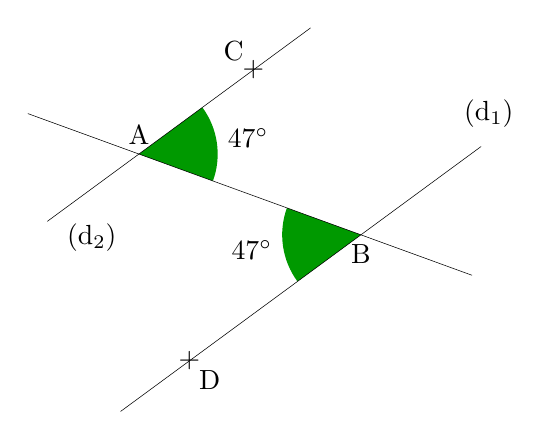
\begin{tikzpicture}[rotate=-20,baseline=(C.base)]
        \coordinate[label=above:A](A)at(0,0);
        \coordinate[label=below:B](B)at(3,0);
        \coordinate[label=above left:C](C)at(1,1.5);
        \coordinate[label=below right:D](D)at(1.5,-2.25);
        \draw node at(C){+};
        \draw node at(D){+};
        \tkzFillAngle[fill=green!60!black](B,A,C)
        \tkzLabelAngle[pos=1.4](B,A,C){$47^\circ$}
        \tkzFillAngle[fill=green!60!black](A,B,D)
        \tkzLabelAngle[pos=1.4](A,B,D){$47^\circ$}
        \tkzDrawLine[add=0.8 and 0.5](A,C)
        \tkzDrawLine[add=0.4 and 0.7](D,B)
        \tkzDrawLines[add=0.5 and 0.5](A,B)
        \draw node at(-0.2,-1.2){(d$_2$)};
        \draw node at(4,2){(d$_1$)};
    \end{tikzpicture}
    \hfill}\hbox{b)%
    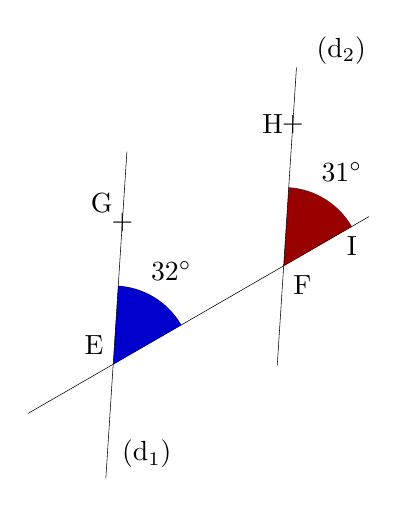
\begin{tikzpicture}[rotate=30,baseline=(C.base)]
        \coordinate[label=above left:E](A)at(0,0);
        \coordinate[label=below right:F](B)at(2.5,0);
        \coordinate[label=below:I](I)at(3.5,0);
        \coordinate[label=above left:G](C)at(1,1.5);
        \coordinate[label=left:H](D)at(3.5,1.5);
        \draw node at(C){+};
        \draw node at(D){+};
        \tkzFillAngle[fill=blue!80!black](B,A,C)
        \tkzLabelAngle[pos=1.4](B,A,C){$32^\circ$}
        \tkzFillAngle[fill=red!60!black](I,B,D)
        \tkzLabelAngle[pos=1.4](I,B,D){$31^\circ$}
        \tkzDrawLine[add=0.8 and 0.5](A,C)
        \tkzDrawLine[add=0.4 and 0.7](D,B)
        \tkzDrawLines[add=0.5 and 0.5](A,B)
        \draw node at(-0.2,-1.2){(d$_1$)};
        \draw node at(4.5,2){(d$_2$)};
    \end{tikzpicture}
    }}
    \question
    Paul va à la boulangerie. Une baguette côute 0,82 \euro. Il achète 5 baguettes et des bonbons pour 2,30 \euro.
    \begin{parts}
        \part Écrire une expression numérique permettant de calculer le montant total des achats de Paul.
        \part Calculer le montant total des achats de Paul.
    \end{parts}
    \question
    Dans une station de ski, on a compté le nombre de personnes qui prennent un remonte-pente.
    \begin{center}
        \begin{tblr}{colspec=*{6}{Q[c,m,wd=30pt]},
            column{1}={wd=100pt,bg=gray!50},hlines,vlines}
            {\bfseries Duréee} (min)&10&20&30&45&50\\
            {\bfseries Nombre de personnes}&8&16&24&35&40\\
        \end{tblr}
    \end{center}
    Le nombre de personnes est-il proportionnel à la durée~?
    \question Une recette de cuisine prévoit 210 g de fromage pour 6 personnes.
    \begin{parts}
        \part Quelle masse de fromage faut-il prévoir pour 14 personnes~?
        \part Combien de personnes peut-on prévoir avec 350 g de fromages~?
    \end{parts}
    Trois amis ont laissés leur voitures sur un parking payant, puis ils ont comparé leurs tickets.
    \begin{center}
        \begin{tblr}{colspec=*{4}{Q[c,m]},hlines,vlines,
            column{1}={bg=gray!50},row{1}={bg=gray!50}}
            \cline{2-4}&Lucas&Emma&Océane\\
            Durée&50 min&1h20 min&2h\\
            Prix&1 \euro&1,60 \euro&2,40 \euro\\
        \end{tblr}
        \begin{parts}
            \part Le prix à payer est-il proportionnel à la durée de stationnement~?
            \part Victoria laisse sa voiture sur le parking à 14h45 et la récupère à 17h15. Combien devra-elle payer~?
        \end{parts}
    \end{center}
    \question Sur cette figure à main levée, les droites (EF) et (GH) se coupent en I.
    \begin{center}
        \includegraphics[scale=2]{G:/Datas/latex/graphics/pdf/5e-Transmath-55-pic.pdf}
    \end{center}
    \begin{parts}
        \part Calculer la mesure de l'angle $\widehat{IGH}$. Justifer.
        \part Calculer la mesure de l'angle $\widehat{IEH}$. Justifer.
        \part Que peut-on dire des droites (EH) et (GF)~? Justifier.
    \end{parts}
    \end{questions}
\end{document}